\chapter{Case Studies in English Diachrony}\label{ch:diachron}
\section{Introduction}
This chapter supports the claims made in the previous three chapters with two case studies in the development of recipient ditransitive syntax in the history of English. The first case study examines changes in the realisation of the dative P head. The second case study examines changes in the morphosyntax of recipient ditransitive passives. As discussed in the introduction, quantitative (and especially) diachronic studies can provide a useful independent verification of analyses developed on the basis of acceptability judgements. Crucially, data from systematic patterns in language production can provide independent verification of theories developed primarily from language comprehension (i.e., acceptability judgements). This chapter begins with an introduction to the quantitative study of historical syntax, focussing primarily on statistical methods of extracting information from quantitative data. This background section is followed by a discussion of each of the case studies mentioned above.

\section{Quantitative Study of Historical Syntax}
	Under the (commonly adopted) Borer--Chomsky Conjecture \citep{Baker.2008}, syntactic variation is driven by features of functional lexical items. Under this system, the syntactic machinery is universal and differences in the lexicon of functional items are the only points of syntactic variation. The presence/absence of a syntactic operation is formally implemented as the presence/absence of a particular feature on a functional head. Thus, syntactic change involves the addition, removal or replacement of functional items in the lexicon.

	Morphological change (especially with respect to allomorphy) can be thought of in similar terms. This analogy can be seen in the Distributed Morphology (DM) formalism \citep{Halle.1993}. In DM, allomorphy is captured by the use of vocabulary items, which formalise the relationship between syntactic/semantic features and phonological forms. Each vocabulary item must contain a set of syntactic/semantic features and a phonological form (e.g., /z/ $\leftrightarrow$ [+pl] for English plurals). A vocabulary can also contain a context in which the vocabulary item applies (e.g., /n/ $\leftrightarrow$ [+pl] / [OX,\dots]$^{\smallfrown}$\_ captures the allomorphy in plural suffixes producing English \textit{oxen}). The Subset Principle of DM (related to Panini's Elsewhere Principle) states that when multiple vocabulary items could apply (for example the contextual conditions of both the regular /z/ and irregular /n/ forms are met with the root OX), the more specific item is used (in this case the irregular /n/ form). Changes in allomorphy, thus, reflect the addition, removal or replacement of vocabulary items.

	Both syntactic and morphological changes have two stages. In order for the change to begin, some language user needs to innovate a new form, in a process called \textit{actuation}. Once a change has been actuated, the new form then needs to spread. Other speakers need to adopt the form, and speakers need to use the form more and more frequently. The increase in use frequency of the forms has been attributed to the process of grammar competition.
	
	Grammar competition occurs when two items compete to fulfil the same pragmatic function. Given that the pragmatic function of the items is the same, a speaker has no a priori way of choosing between the two items. This creates a situation of grammar competition, where two equal (or nearly equal) options are competing for use in speakers productions \citep{Kroch.1989}. \cite{Wallenberg.2013} discussed how these cases either end with one of the options driving out the other, or in specialisation, where the two options subdivide the pragmatic space and each become the unique representative of their own smaller space. A frequent outcome of this competition, diachronically, is that a newer alternatives replaces an older alternative, i.e., that over time the probability of the newer alternative continuously increases at the expense of the older alternative. Note that while the two alternatives reflect differences within the grammatical system, after the new alternative is innovated, the remaining change occurs within the non-grammatical system (i.e., is a change in the probability distribution over grammatical alternatives).

	These changes have been traditionally studied (since \citealt{Kroch.1989}) using \textit{logistic regression}, which is the standard statistical method to study variation in probabilities (i.e., numbers that range from 0 to 1). For syntactic change, the relevant probabilities are the probability of the surface form produced by the new item in any given year/context (i.e., the number of examples of the new form produced in a given year divided by the total number of opportunities to use either the old or new form). Year usually reflects the year the text was composed (assuming that the text is representative of the language for that year). The contexts reflect other factors that influence the probability of the different possible items being used (e.g., the pronoun vs. full noun status of arguments).

	Logistic regression maps the log odds\footnote{For any probability $p$, the log odds are defined as $log(\frac{p}{1-p})$.} (which range from -$\infty$ to $\infty$) to probabilities (which range from 0 to 1) using the following function: $p=\frac{1}{1+\text{exp}(-(\text{log odds}))}$. The log odds can then be modelled using linear regression, which is a modelling problem that has well understood methods for fitting to data. Linear regression models the value of a dependent variable (e.g., height) as the sum of weighted independent variables (e.g., age and gender). The weighting is done by multiplying each of the independent variables by a constant (called a regression coefficient). The goal of linear regression is to find the value for the regression coefficients that causes the sum of the weighted independent variables to best predict the dependent variable (for the data being modelled).

	There are three relevant types of regression coefficients for quantitative investigation of syntactic change using logistic regression. All models include an \textit{intercept}, which (for logistic regression) captures the average probability when all of the dependent variables are zero (for syntactic change this usually means for year 0 for some subset of syntactic contexts). The next type of regression coefficient are \textit{simple effects}, which for syntactic change indicate the effect of moving from one year to the next or from one context to another. The final type of regression coefficient are \textit{interactions}, which for syntactic change indicate how either the effect of year is different between different contexts or how the effect of one context is different based on some other context (e.g., how the effect of the recipient being a pronoun may be different depending on whether the theme is a pronoun or a full noun phrase).

	One of the major discoveries coming from the quantitative study of diachronic syntax has been the Constant Rate Effect \citep{Kroch.1989,Kroch.1994}. This effect obtains when considering a change that applies in multiple syntactic contexts. In these cases, it has been repeatedly found that the effect of year fit by logistic regression is constant across its different syntactic contexts (this is true even in cases where the environments themselves show different frequencies of use). Practically speaking, this means that significant interactions between year and variables representing syntactic contexts are not found.

	Note that the Constant Rate Effect relies on detecting a null effect (i.e., the \textit{absence} of a significant interaction). There is a statistical problem with interpreting the lack of a significant interaction in the model as reflecting a lack of interaction in reality, namely that all the statistical test can do is indicate whether there is sufficient data to reject the null hypothesis (i.e. that there is no interaction in reality). Thus, the lack of a significant interaction could reflect either: (a) the absence of an interaction in reality or (b) the absence of enough data to detect a real interaction. One solution to this problem is to take two further steps: (i) decide how large an effect would need to be to be considered substantial\footnote{It would take an infinite amount of data to detect that an interaction is exactly 0. However, if the effect of the interaction is really 0.00001, it would be safe to conclude that the interaction is practically non-existent. Here judgement is necessary to decide what size effect should be considered large enough that it would not be reasonable to ignore it.} and (ii) demonstrate that the data is sufficient to detect an interaction of that size. If the data set is at least as large as determined in (ii) and an interaction is still not detected, the conclusion can then be drawn that the interaction is unlikely to be substantial enough to count as a counterexample to the Constant Rate Effect.

	The first example of the Constant Rate Effect comes from \cite{Kroch.1989}, where the use of do-support was studied in a number of different environments (e.g., negative declaratives, affirmative questions, negative questions, imperatives, etc.). Kroch found that while the frequency of the use of do-support in these environments differed from one another in any given year (see Fig. \ref{fig:kroch-graph}), the rate at which these frequencies changed was constant across environments (i.e., there was no significant interaction between year and the variables representing the different contexts of do-support). He hypothesised that this effect reflected the fact that only one change was taking place (the loss of V-to-T raising). Under this hypothesis, the Constant Rate Effect provides a means of recovering underlying grammatical information from diachronic patterns in language use. If a Constant Rate Effect is found (assuming that one has enough data that it would be possible to fail to find it), the most parsimonious hypothesis is that a unified change underlies the variation in each environment (i.e., use of a single new functional item is increasing in frequency).

	\begin{figure}[ht!]
		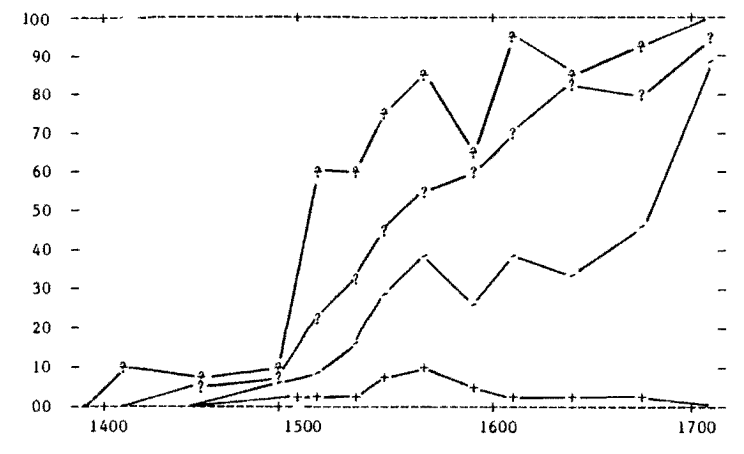
\includegraphics[width=.5\linewidth]{../images/kroch-graph}
		\caption{Frequency of do-support in different environments: affirmative and negative questions (? and \sout{?}) and affirmative and negative declaratives (+ and ') (Fig. 1 from \citealt{Kroch.1989})}
		\label{fig:kroch-graph}
	\end{figure}

\section{Recipient Marking}
\subsection{Dative P Allomorphy}
This section shows how data from the history of English supports the allomorphy analysis of dative shift. As discussed in Chapter \ref{ch:active}, dative shift is the modern English phenomenon, where the recipient is unmarked when adjacent to the verb (e.g., ``John gave Mary the ball''), but marked with `to' elsewhere (e.g., ``John gave the ball to Mary''). This can be captured with the pair of vocabulary items in (\ref{ex:eng-ds-vi}). This section shows how this grammar arose in the history of English. In order to support the claim that the absence of recipient marking in sentences like ``John gave Mary the ball'' reflect null allomorphy of the P head, I report a finding of the Constant Rate Effect. In particular, I provide evidence for a uniform To Item across all recipient contexts.  

	\begin{exe}
		\ex \label{ex:eng-ds-vi}
		\begin{xlist}
			\ex Null Allomorph Item: /$\emptyset$/ $\leftrightarrow$ [dative P] / verb$^{\smallfrown}$\_
			\ex To Item: /tu/ $\leftrightarrow$ [dative P]
		\end{xlist}
	\end{exe}


	Neither of the vocabulary items in (\ref{ex:eng-ds-vi}) were inherited from Old English. Old English had synthetic dative case marking, where the dative P head was realised as null (\ref{ex:old-eng-vi}), but its features were copied onto elements of the noun phrase through concord and realised on determiners, adjectives and noun heads as synthetic dative case. A consequence of the concord is that even though dative P was itself not realised phonologically, its features were phonologically realised on elements in the noun phrase. 
	
	\begin{exe}
		\ex \label{ex:old-eng-vi}
		\begin{xlist}
			\ex Null Item:  /$\emptyset$/ $\leftrightarrow$ [dative P]
		\end{xlist}
	\end{exe}
	
	By the end of the Old English period (11th century), the morphological distinction between accusative and dative case was breaking down. Case marking on nouns, adjectives and determiners was no longer reliable. Both accusative and dative pronominal forms were still being used, but the forms were no longer consistently associated with dative and accusative case (i.e., old dative case forms would be used where previously accusative case was required and vis-a-versa). Around this time, `to' began to be used for the first time to introduce recipients. In Old English, `to' had previously been restricted to goals and addressees, i.e., the indirect object of verbs of communication \citep{Allen.1999,McFadden.2002,OED.2013}. 
	
	The fact that `to' began to be used at this point, once all overt realisation of dative P was lost, suggests that language learners are predisposed to look for an overt realisation for syntactic/semantic features. Null realisation of non-root morphemes is compatible with any surface form, since variation in form can be attributed to allomorphy of more inward elements (e.g., /dogz/ + $\emptyset$ is a compatible grammatical model for English plurals, realising DOG+[+PL]). Thus, language learners must have a heuristic that favours overt realisation and posits null forms as a last resort. The outcome of this heuristic can be seen here, where a new overt form was innovated within a generation or two of the loss of the final remnants of the old overt forms. 

	The first change in recipient marking was the introduction and spread of the To Item. The new grammar of English after the introduction of the To Item is shown in (\ref{ex:simple-vis-eng}). Since neither of the vocabulary items are more specific than the other, and both realise the same syntactic/semantic features, the grammar is unable to determine which item to use, which is the classic situation of grammar competition.

	\begin{exe}
		\ex \label{ex:simple-vis-eng}
		\begin{xlist}
			\ex Null Item: /$\emptyset$/ $\leftrightarrow$ [dative P]
			\ex To Item: /tu/ $\leftrightarrow$ [dative P]
		\end{xlist}
	\end{exe}


	In order to quantitatively study changes in the use of `to' for dative P, I extracted all tokens from the Parsed Corpora of Historical English \citep{Kroch.2000,Taylor.2003,Kroch.2004,Taylor.2006,Kroch.2010} containing the following recipient introducing verbs (verbs that also introduce goals, e.g., SEND, were excluded): ALLOT, APPOINT, ASSIGN, AYEVEN, BEHIEGHT, BEQUEATH, BETAKE, DAELAN, FEED, GIVE, GRANT, LEND, OFFER, OWE, PAY, PROFFER, PROMISE, RESTORE, SELL, SELLAN, SERVE, SHOW, VOUCHSAFE, and YIELD. I also extracted information about whether the arguments were full noun phrases or pronouns, the relative order of the recipient and theme (and their order with respect to the verb to rule out cases of topicalisation), and whether or not the recipient was marked with `to' (passive data was also collected, which is discussed in Section \ref{sec:en-pas}).\footnote{See Appendix A for links to the queries used in collecting this data.}

	The availability of cliticisation makes data from theme pronouns more complicated, so I leave their discussion till the next subsection. Here, I focus on cases with full noun phrase themes (e.g., ``John gave Mary the book''). Looking at data from the period before 1400, rates of `to' use increase in all contexts (see Figure \ref{fig:to-use-bf-1400}). As shown in Chapter \ref{ch:active}, the rise in recipient--theme orders (e.g., ``John gave to Mary the book'') cannot be attributed to Heavy NP shift, but must reflect underlying use of `to' in recipient--theme orders. The claim that the rise in `to' use (even in recipient-theme contexts) reflects the uniform adoption of the To Item would be supported if a Constant Rate Effect was found between the rise in the use of `to' in the recipient--theme and theme--recipient contexts.

	\begin{figure}[ht!]
		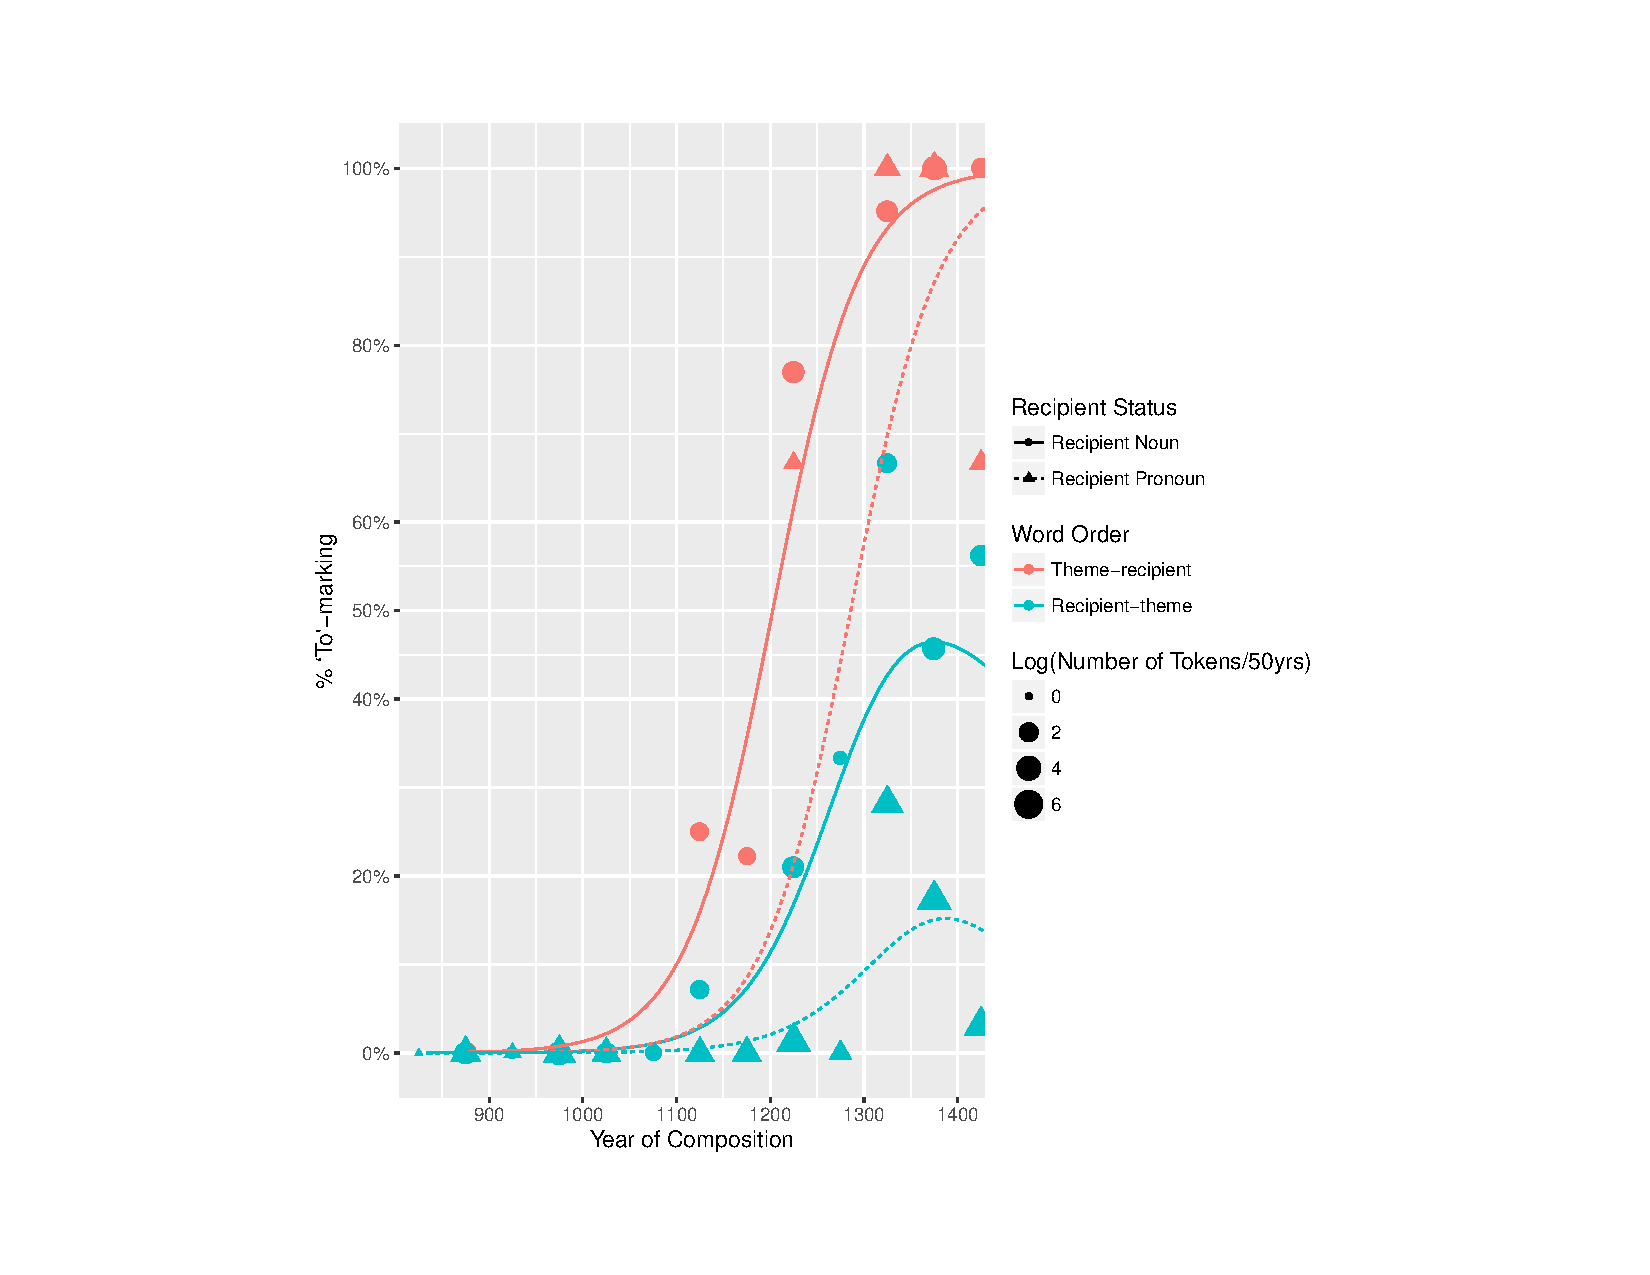
\includegraphics[width=\linewidth]{../images/to-use-bf-1400}
		\caption{Logistic regression models fit to data with theme--recipient word order and full noun phrase themes before 1400}
		\label{fig:to-use-bf-1400}
	\end{figure}

	However, testing for the Constant Rate Effect in this case is non-trivial, since another change occurs simultaneously with the spread of the To Item, namely the introduction and spread of the Null Allomorphy Item (which requires the null realisation if the dative P head is adjacent to the verb). The introduction of this vocabulary item blocks the use of `to' in recipient--theme contexts, since the Null Allomorphy Item is more specific (\ref{ex:eng-ds-vi}). In this case, the two items are not in competition, since they are both compatible within the same grammar (i.e., the grammar knows how to distribute the two forms).

	\begin{exe}
		\exr{ex:eng-ds-vi}
		\begin{xlist}
			\ex Null Allomorph Item: /$\emptyset$/ $\leftrightarrow$ [dative P] / verb$^{\smallfrown}$\_
			\ex To Item: /tu/ $\leftrightarrow$ [dative P]
		\end{xlist}
	\end{exe}

	The relationship between the Null Item and the Null Allomorphy Item also does not lead to grammar competition (\ref{ex:all-null}). In this case, the Null Allomorphy Item is redundant, since the dative P would be realised as null anyway. If these were the only two Items under consideration, there would be no reason to posit the Null Allomorphy Item, so such a grammar would not be learned. However, the grammar does not present a case of grammar competition, since both Items have clearly defined regions of application, and their redundancy is merely incidental (i.e., the structural properties of this grammar are identical to the one in Ex. \ref{ex:eng-ds-vi}).

	\begin{exe}
		\ex \label{ex:all-null} 
			\begin{xlist}
				\ex Null Allomorphy Item: /$\emptyset$/ $\leftrightarrow$ [dative P] / verb$^{\smallfrown}$\_
				\ex Null Item:  /$\emptyset$/ $\leftrightarrow$ [dative P]
			\end{xlist}
	\end{exe}

	Therefore, the Null Allomorph Item is not replacing any item currently in the system (i.e., it is not in competition with either the To Item or the Null Item). Instead, what needs to be modelled is the adoption of this item into the grammar. In other words, the Null Allomorphy Item is in competition with its own absence, rather than any item currently in the system. Presumably, the adoption of the Null Allomorphy Item is subject to the same historical pressures as any other morphosyntactic change (i.e., that the change must be gradual enough that speakers of contemporaneous generations can understand each other). I therefore assume that it can be modelled using the same logistic regression models used in classical cases of grammar competition.

	Before returning to the question of how to model the relationship between the To Item and the Null Allomorph Item, it seems worthwhile to note that the actuation of the Null Allomorph Item has a clear explanation in this case. As seen in Figure \ref{fig:to-use}, `to' use declines in recipient--theme orders (blue lines) around the same time that `to' becomes categorical (or nearly categorical) in theme--recipient orders (red lines). Thus, children were exposed to primary linguistic data produced by parents who had a grammar consisting of the To Item and the Null Item (\ref{ex:adult-grammar}), but whose probabilistic use of the To Item and Null Item in the theme--recipient and recipient--theme contexts was consistent with a grammar containing the To Item and the Null Allomorphy Item (\ref{ex:child-grammar}). Once the Null Allomorphy Item had been innovated, it then needed to spread (i.e., it needed to compete with grammars that lacked the Null Allomorphy Item).

	\begin{exe}
		\ex Adult Grammar:\label{ex:adult-grammar}
		\begin{xlist}
			\ex Null Item:  /$\emptyset$/ $\leftrightarrow$ [dative P]
			\ex To Item: /tu/ $\leftrightarrow$ [dative P]
		\end{xlist}
		\ex Child Grammar:\label{ex:child-grammar}
		\begin{xlist}
			\ex Null Allomorphy Item: /$\emptyset$/ $\leftrightarrow$ [dative P] / verb$^{\smallfrown}$\_
			\ex To Item: /tu/ $\leftrightarrow$ [dative P]
		\end{xlist}
	\end{exe}

	\begin{figure}[ht!]
		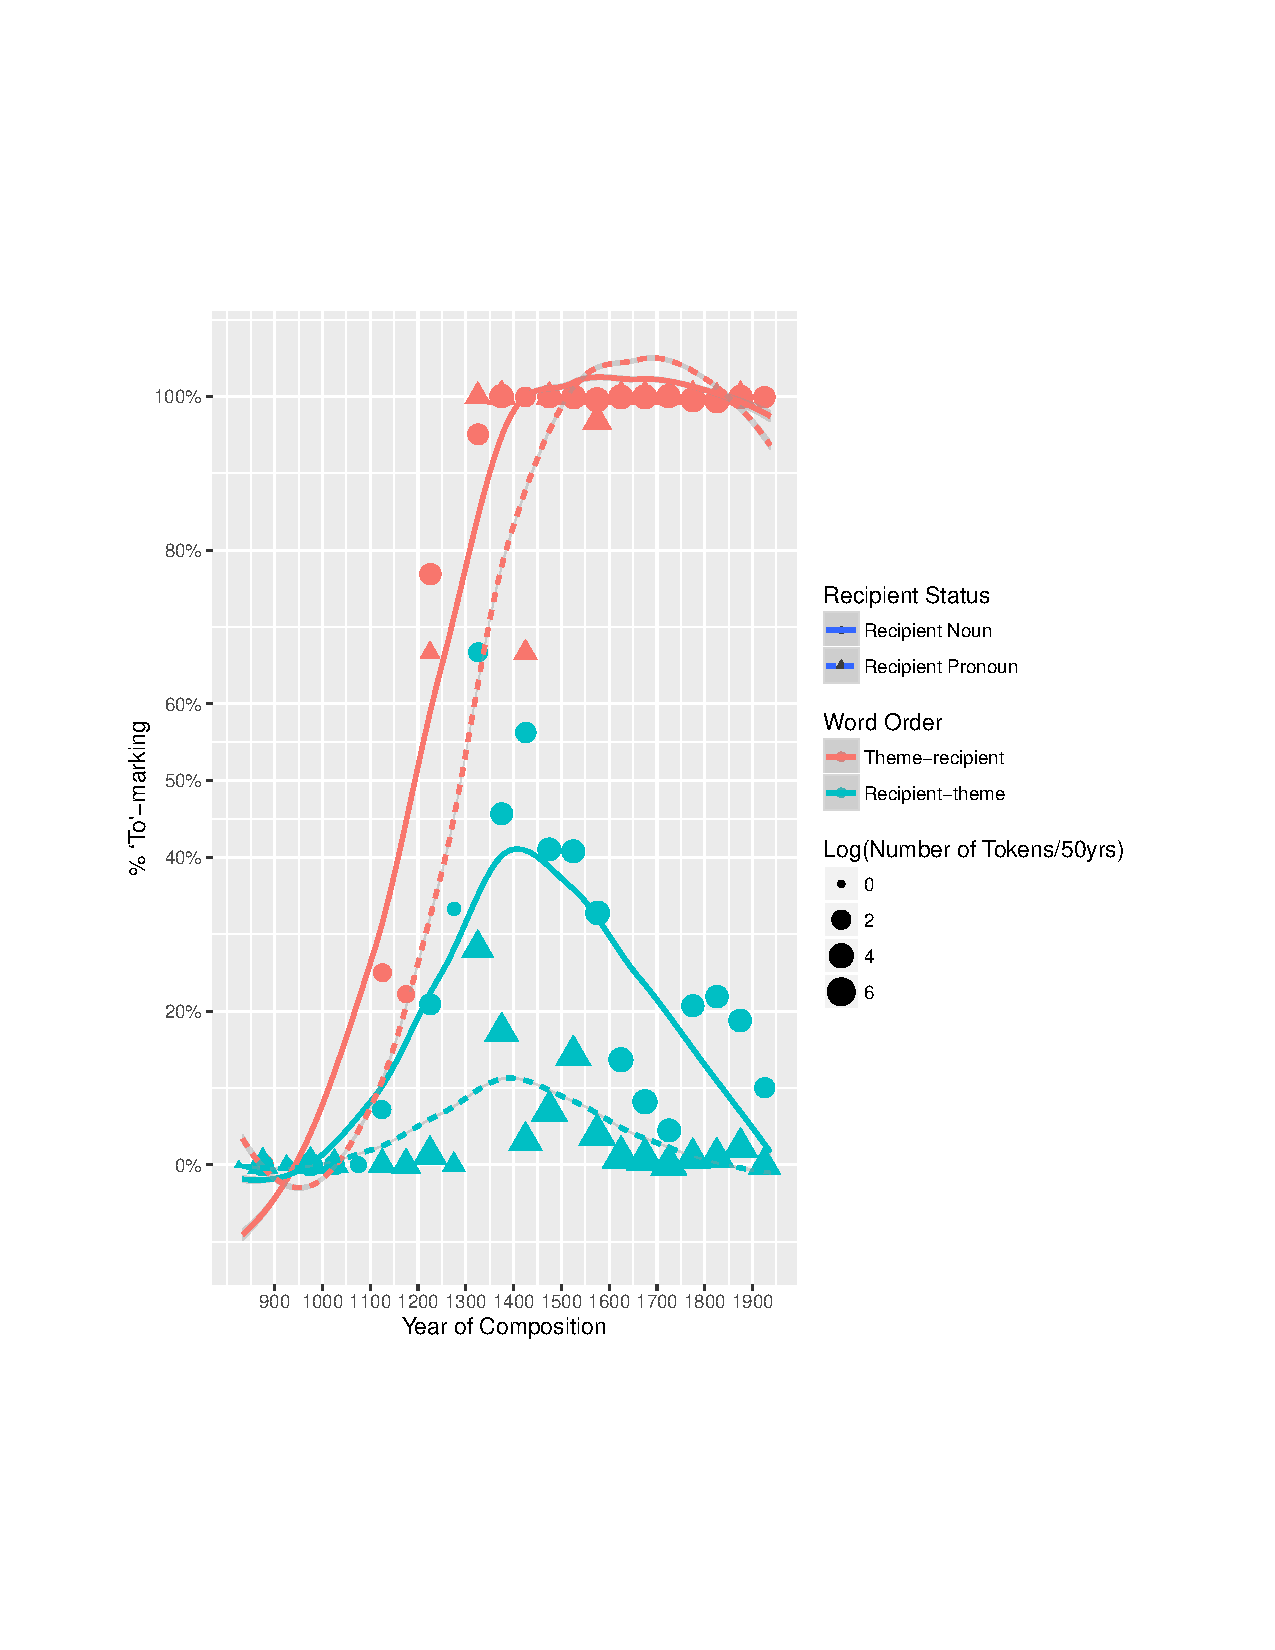
\includegraphics[width=\linewidth]{../images/brit-tn}
		\caption{Logistic regression models fit to data with theme--recipient word order and full noun phrase themes}
		\label{fig:to-use}
	\end{figure}

	Bringing the two changes together (the competition between the To Item and the Null Item and the spread of the Null Allomorphy Item) allows for a simple statistical model for the rate of `to' use. Both changes can be modelled using simple logistic regression, where the dependent variable for one model is the probability of using the To Item and the dependent variable for the other model is the probability of including the Null Allomorphy Item. For each change, a Constant Rate Effect can be tested. The first change has four different contexts of application that the Constant Rate Effect can be tested over: (i) pronoun recipient recipient--theme, (ii) pronoun recipient theme--recipient, (iii) full noun recipient recipient--theme and (iv) full noun recipient theme--recipient. The second change is restricted to recipient--theme orders, since the inclusion/lack of the Null Allomorphy Item does not impact the use of `to' in theme--recipient orders, since the P head is not adjacent to the verb. 

	In order to fit these two logistic regressions, it is necessary to map the probability of each change occurring to the probability of `to' use, since the only data available is the rate of `to' use in various contexts. As discussed in the previous paragraph, the second change does not impact `to' use in the theme--recipient context, so the theme--recipient context can be modelled directly by using the logistic regression from the first change. For the recipient--theme context, however, the rate of `to' use is equal to the probability of using the To Item and not including the Null Allomorphy Item (as can be seen by the distribution of `to' in Table \ref{tab:2x2int}). Assuming that the two changes are independent, basic statistics states that the probability of two independent events occurring is equal to the product of the probability of the two independent events. In other words, the probability of `to' in recipient--theme contexts is equal to the probability of the To Item times 1 - the probability of including the Null Allomorphy Item (i.e., the probability of not including the Null Allomorphy Item). Thus, we can fit the data by using a model that multiples the two logistic equations together and fits the data to that model (see Appendix A for details on how this fitting occurred).

	\begin{table}[ht!]
		\begin{tabular}{ccc}
					& No Null Allomorphy Item & Null Allomorphy Item\\
			Null Item	& John gave Mary the book & John gave Mary the book\\
			To Item 	& John gave \textbf{to} Mary the book & John gave Mary the book\\
		\end{tabular}
		\caption{2x2 table showing the interaction between the two changes in dative P realisation in English in recipient--theme contexts}
		\label{tab:2x2int}
	\end{table}

	A single model was fit that predicted both the theme--recipient and recipient--theme orders for data with full noun phrase themes using the multiplication model discussed in the previous paragraph. The full model for each change contained effects for year, recipient type, and object order as well as their interactions. The optimal model was selected to have the lowest AIC.\footnote{AIC, Akaike Information Criterion, is a way of selecting models that fit the data well, while taking into account the fact that adding more independent variables always improves fit. Comparing AIC, selects the model that finds an optimal balance between fitting well and having few independent variables.} 
	
	The optimal model had the following properties (model fits shown above in Fig. \ref{fig:to-use}): (a) the first change was characterised by an intercept, an effect of year, an effect of word order and an effect of recipient status, (b) the second change was characterised by an intercept, an effect of year, and effect of recipient status, and an interaction between year and recipient status. The effects in model (a) indicate a Constant Rate Effect for the introduction of `to'-marking for recipients; there was no significant interaction between conditions. While `to'-marking raises at the same rate across all conditions, recipient--theme orders and recipient pronouns show less `to'-use in any given year. 
	
	As discussed above, failing to find a significant interaction is not enough to automatically claim that the Constant Rate Effect was found, it is possible that there was insufficient data to find a substantial violation of the Constant Rate effect. This explanation for the Constant Rate Effect finding in the first change (adoption of To Item) becomes less plausible, given that a significant interaction was identified for the second change (adoption of the Null Allomorphy Item) indicating that there was enough data to identify interactions. The identification of a significant interaction for the second change strongly suggests that there are actually two Null Allomorphy Items (one for recipient nouns and one for recipient pronouns). The effect of year was found to be higher for recipient pronouns, suggesting that the Allomorphy Grammar affected recipient pronouns faster than full noun phrases (meaning more null forms for pronouns).
	
	Since many languages have a strong differentiation between recipient marking on full noun phrases and pronouns (e.g., Romance language differences between full noun phrases marked with \textit{a} `to' and clitic pronouns marked with synthetic case marking), this differentiation between full noun phrases and pronouns is not unexpected. It appears that there are actually two Null Allomorphy Items: one that applies to nouns, and another that applies to pronouns, which both have the same output, namely $\emptyset$, but which spread through the speech community at different rates. The grammar for pronouns rapidly spread through the speech community (possibly influenced by the fact that pronouns maintained some level of synthetic case marking), while the grammar for full noun phrases spread more slowly. This can be seen above in Figure \ref{fig:to-use}, where the pronouns show a much less `to' use overall compared to full noun phrases (in recipient--theme word orders).

	\begin{exe}
		\ex 
		\begin{xlist}
			\ex Pronoun Null Allomorph Item: /$\emptyset$/ $\leftrightarrow$ [dative P] / verb$^{\smallfrown}$\_$^{\smallfrown}$pronoun
			\ex Null Allomorph Item: /$\emptyset$/ $\leftrightarrow$ [dative P] / verb$^{\smallfrown}$\_
			\ex To Item: /tu/ $\leftrightarrow$ [dative P]
		\end{xlist}
	\end{exe}


	By modelling overlapping changes by multiplying their independent probabilities, it was possible to confirm another case of the Constant Rate Effect. In this case, the Constant Rate Effect applied to the rise of the To Grammar. Given that there was independent support that the data was sufficient to detect meaningful interactions, there is solid evidence that the adoption of the To Item was a unified change that applied during the Middle English period. As discussed in Chapter \ref{ch:active}, this supports the dative PP hypothesis by bolstering the notion that the `to' found in the modern theme--recipient orders is actually shared by the recipient--theme order. The multiplication model also identified two different grammatical processes for generating unmarked nouns and pronouns, a differentiation which could only be discovered by using quantitative data, since the outputs of the items are identical.

	\subsection{More on Pronoun Cliticisation}
	In this subsection, I present more evidence of special behaviour by pronouns, focusing of data where the theme is a pronoun. When the theme is a pronoun, the theme--recipient order was essentially categorical (31 examples of recipient--theme order over 1000 years out of 712 examples with theme pronouns). Since there was such poor evidence for the frequency of `to'-use in these environments, their inclusion muddled any attempts at statistical analysis. Therefore, those cases have been excluded for the analyses discussed below. Instead, I focus on cases where with a theme pronoun and a theme--recipient order.

	As discussed in Chapter \ref{ch:active}, theme pronoun cliticisation can produce surface violations of the generalisation that the null allomorph of the dative P head only occurs adjacent to the verb (e.g., ``John gave it Mary''). The theme pronoun does not intervene once it has cliticised, because it is considered morphologically to be a part of the verb. I showed that in some dialects of Northwestern British English, this process was still occurred:

	\begin{exe}
		\exr{ex:nw-brit-P} Northwestern British English:
		\begin{xlist}
		\ex[ ]{John [gave=it] [P=$\emptyset$ Mary]}
		\ex[*]{John [gave] [the book] [P=$\emptyset$ Mary]}
	\end{xlist}
	\end{exe}

	The effect of theme pronoun cliticisation can also be seen in the historical data. Figure \ref{fig:brit-tr} shows data from theme--recipient word orders with theme pronouns. In both cases, the same rise in `to' as discussed earlier is seen, which just shows the adoption of the To Item. However, instead of levelling out at 100\%, for both recipient noun phrases and recipient pronouns, the logistic regression goes to some point short of completion, which can be explained as reflecting the combination of adopting the Null Allomorphy Item and the rate of theme pronoun cliticisation. For full noun phrase recipients, the rate of `to' use is $\sim$93\%, while for pronoun recipients, the rate of `to' use is $\sim$42\%.\footnote{These reflect the average rate of `to' use in these two context between 1425 and 1700.} While theme pronoun cliticisation explains the existence of null marked recipients in these contexts, it does not explain the discrepancy between full noun phrase and pronoun recipients.

	\begin{figure}[ht!]
		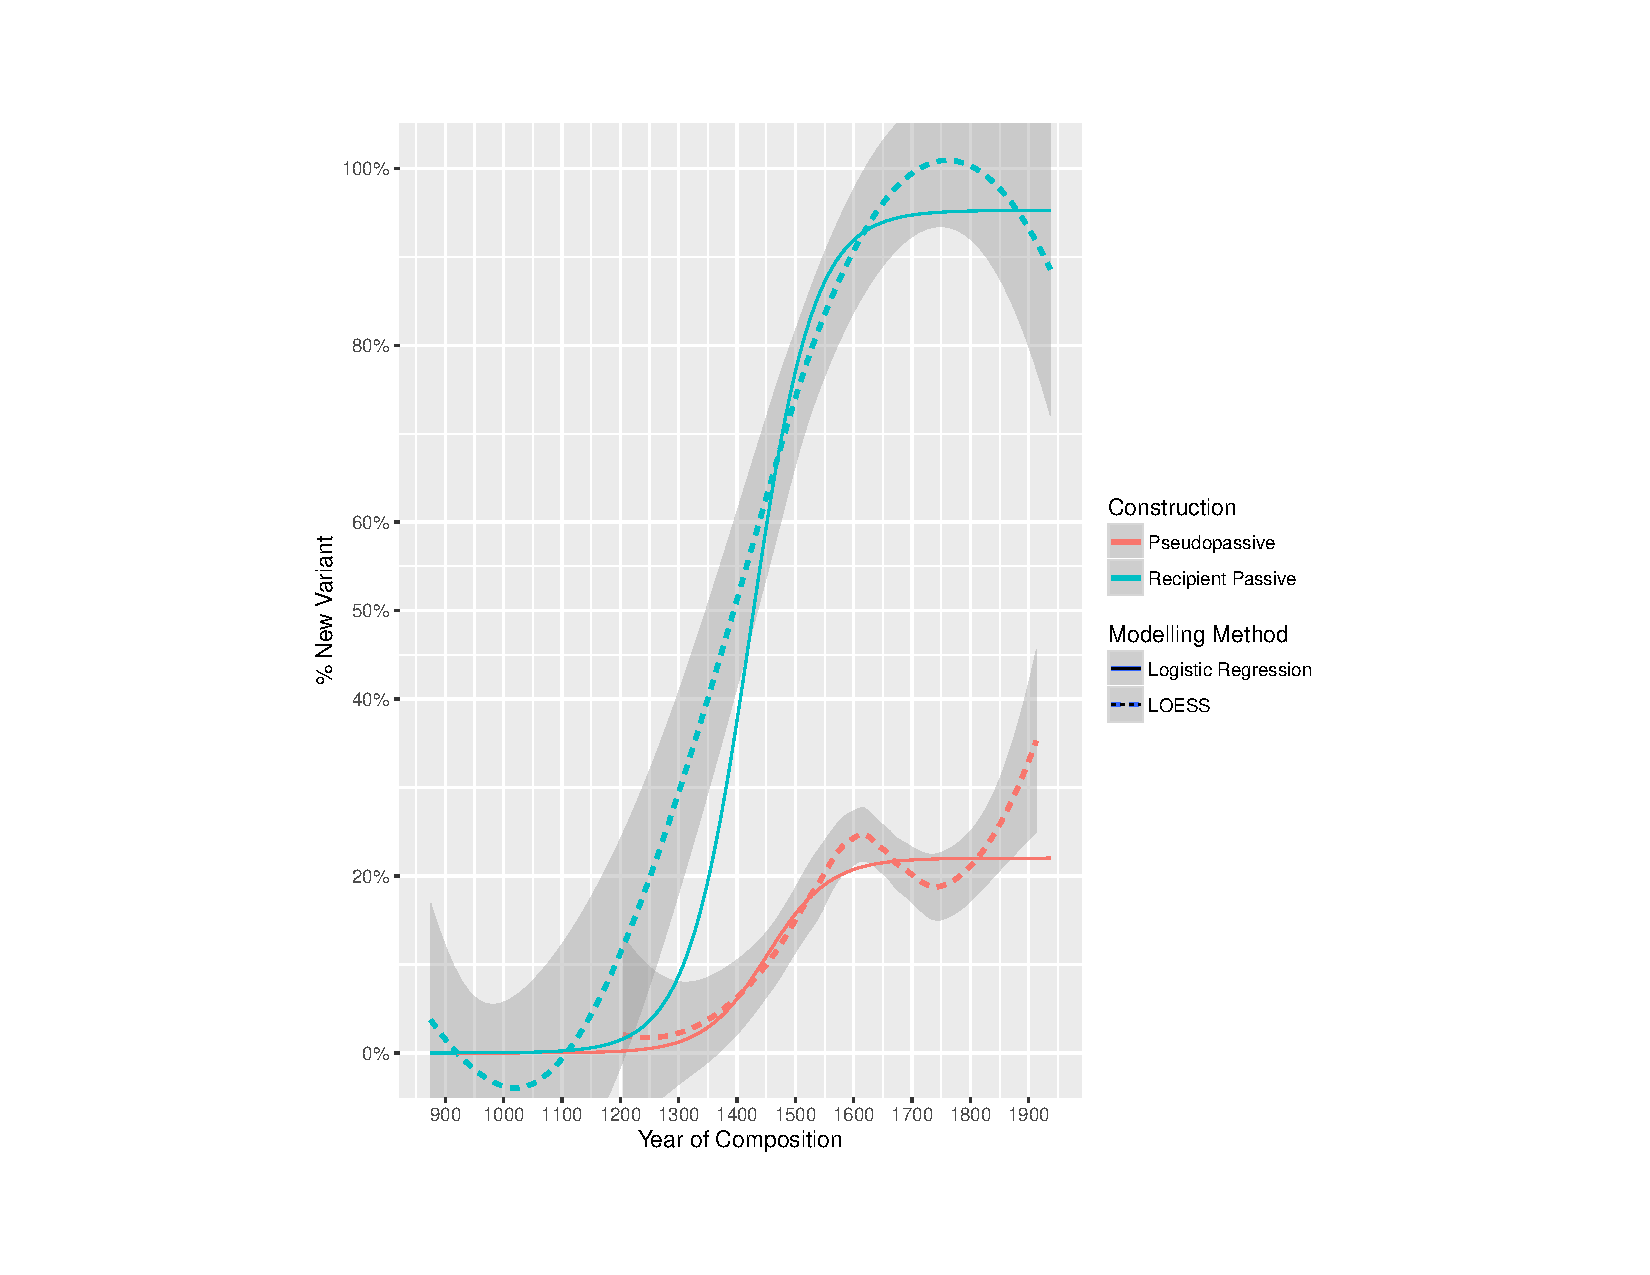
\includegraphics[width=\linewidth]{../images/brit-tp}
		\caption{LOESS fits for theme--recipient data with theme pronouns (points indicate raw frequencies)}
		\label{fig:brit-tr}
	\end{figure}

	In the previous subsection, it was seen that pronoun recipients showed different behaviour from full noun phrase recipients in the adoption of the Null Allomorphy Item. I proposed that this involved a process of recipient pronoun cliticisation, which showed different morphological marking than full noun phrase recipients. The same explanation works for the situation discussed here. Theme cliticisation on its own is fairly rare, as seen by the low rate of null full noun phrase recipients. However, when both the theme and the recipient are pronouns, both pronouns are likely to cliticise, and the null form associated with the recipient pronoun explains the lower rates of `to' use. The propensity for recipient pronouns to be null marked seen both in this subsection and the previous subsection supports the notion that the use of `to' reflects morphological variation that is sensitive to pronominality as is seen in the morphological distinction between clitic and non-clitic pronouns in many Romance varieties.

	As can be seen in Figure \ref{fig:brit-tr}, the difference between pronouns and full noun phrases seems to be shrinking in standard Modern British English (i.e., after 1700). As discussed in chapter \ref{ch:passive}, American English data shows that sentences like ``John gave it Mary'' and ``John gave it him'' were already rare at the beginning of the 19th century in American English and were lost by the middle of the 20th century. While the British data ends in the early 20th century, it seems that the same process was affecting standard British English. It seems both standard British and standard American English lose pronoun cliticisation effects over the 18th, 19th and 20th centuries.
	
	\section{Passivisation}\label{sec:en-pas}

	This section deals with quantitative data on passivisation with recipient ditransitives, which I argue includes a case of non-grammatical change (i.e., a systematic change in use that does not reflect any change in the underlying grammar). In order to justify this claim, I start by showing that the situation in Old English is ambiguous and thus worth setting aside. I then show two grammatical changes with respect to passivisation of ditransitive recipients: (a) replacement of oblique recipient subjects with nominative recipients and (b) the loss of direct theme passivisation in American English, where direct theme passivisation is reflected in sentences like ``The book was given John''. Finally, I show how the rate of passivisation of ditransitives with recipient--theme word order changes in American English and argue that this change should not be attributed to a change in underlying grammar, but instead to a change in the way speakers choose between multiple possible grammatical utterances. 

\subsection{Old English}
	The situation in Old English is quite complex. \cite{Allen.1999} provides evidence that monotransitive datives are able to become oblique subjects in Old English, but she suggests that in ditransitives, putative oblique subjects are actually topics. To discuss this distinction, she introduces the term ``fronted dative'', which is agnostic as to whether the fronted element is a topic or a subject. The argument about the status of fronted datives in ditransitive passives is made on the basis of Coordinate Subject Deletion facts. In Old English (as in Modern English), arguments are generally obligatory (i.e., neither subject nor object drop is generally licensed). However, when two sentences are coordinated and share the same subject, the subject does not need to be expressed in the second sentence (\ref{ex:OECSD}). In a corpus investigation, none of the fronted datives in ditransitive passives triggered Coordinate Subject Deletion, while a number of fronted nominatives did (see Table \ref{tab:AllenOECSD}). 

	\begin{table}[t]
		\begin{tabular}{cccc}
			Nominative Coreferential & & Deletion & No Deletion \\
			& Order NOM DAT & 11 & 4 \\
			& Order DAT NOM & 4 & 3 \\
			& Total & 15 & 7 \\
			\hline
			Dative Coreferential & & Deletion & No Deletion \\
			& Order NOM DAT & 0 & 27 \\
			& Order DAT NOM & 0 & 11 \\
			& Total & 0 & 38 \\
		\end{tabular}
		\caption{Allen's counts of Coordinate Subject Deletion with ditransitive passive in OE prose (Table 2-6, \citealt{Allen.1999})}
		\label{tab:AllenOECSD}
	\end{table}

	\begin{exe}
		\ex \label{ex:OECSD} Old English:
		\gll and him comon \textbf{englas} to, and him ðenodon\\
		and him.DAT came \textbf{angels.NOM} to, and him.DAT served\\
		\trans ` and to him angels came and him (they) served \citep[ex. 34]{Allen.1999}.''
	\end{exe}

	The main problem with this conclusion is that there were only a small number of Old English coordinated examples, such that the lack of deletion for datives could be accidental. The problem of whether fronted oblique elements are subjects is not unique to Old English. The same uncertainty hold with respect to Old Norse (see for example \citealt{Kristoffersen.1991,Kristoffersen.1994} and \citealt{Bardal.2001b}). Unfortunately, many of the examples that clearly show that oblique elements are subjects rely on negative data, which is unavailable for earlier states of the language. Because of this problem, I focus instead on data starting with Middle English, where I make the assumption that oblique fronted elements are subjects, since Middle English has developed an obligatorily filled subject position.

	\subsection{Changes to Grammar}

	There are two changes going from Early Middle English to Modern American English that affect the grammar of recipient ditransitive passivisation. As discussed in the introduction to this chapter, a grammar distinguishes between strings that are associated with at least one meaning (grammatical strings) and strings that have no association with a meaning (ungrammatical strings). A change to the grammar, thus, means that some strings need to move from one category to another.\footnote{Another type of change in grammar would be a change in the association between meanings among grammatical strings. A grammatical string could be associated with a new meaning, or loose an association with an old meaning, while still being grammatical (i.e., still having some possible interpretations associated with it).} Concerning the passivisation of recipient ditransitives, the two changes are: (a) oblique recipient subjects vs. nominative recipient subjects and (b) availability of direct theme passivisation vs unavailability of direct theme passivisation. 

	As discussed in the previous subsection, I am assuming that Middle English has oblique subjects in cases of fronted recipients. However, since synthetic case marking had been lost (for full noun phrases) by Early Middle English and since the To Grammar (see the previous section) was not yet universal, even with these assumptions, it is difficult to determine whether a fronted recipient was nominative or dative. \cite{Allen.1999}, after carefully examining the extant Middle English corpus, identifies that the first unambiguous case of a nominative recipient subject in the passive of a ditransitive occurs in 1375. This reflects a change in the grammar of English, in so far as previously nominative recipient subjects were ungrammatical and now they are grammatical.

	Under the analysis described in Chapter \ref{ch:passive}, the nature of this grammar change reflects the availability of P-incorporation. Without P-incorporation, the only possible form of recipient passivisation is to have oblique subjects. Given that P-incorporation also generates pseudopassives, the simple prediction would be that pseudopassives would enter the language at the same time as nominative recipient passives. \cite{Sigursson.2014} showed that pseudopassivisation comes into the language in the beginning of the Middle English period. Indeed, as seen in Figure \ref{fig:recpas-pseudo}, pseudopassivisation and nominative recipient passivisation increase in use from about 1200 until 1650, when they both level off.

	\begin{figure}[ht!]
		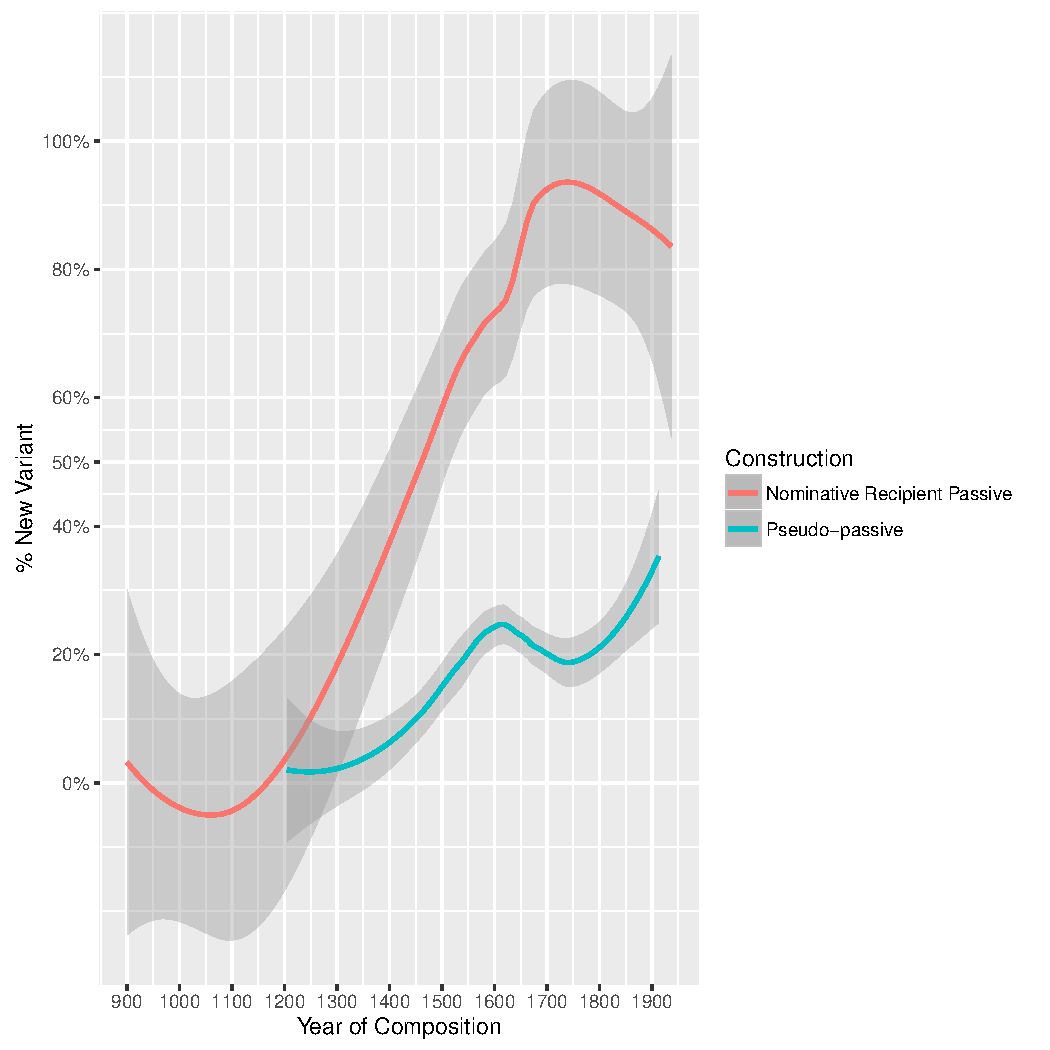
\includegraphics[width=\linewidth]{../images/recpas-pseudo}
		\caption{LOESS curves showing rates of nominative recipient passivisation and pseudopassivisation in English}
		\label{fig:recpas-pseudo}
	\end{figure}

	Neither pseudopassivisation nor nominative recipient passivisation go to 100\%. For pseudopassivisation, this is expected. If the pseudopassivisation rate was 100\% that would mean that there were no active sentences with PP objects, which is highly improbable. For nominative recipient passivisation, it is less clear why the process should not go to completion, since this is the probability of having a nominative subject given that recipient passivisation has occurred, which could reasonably occur 100\% of the time. However, two residual cases prevent this from occurring. Looking at the examples of oblique recipients from the period after 1500, almost all of them are imperatives of the form ``To X, be this given/sent/delivered'', which seem to have been a common formula for deliveries. The other case is locative inversion, for which there is disagreement in the literature about the correct analysis. It seems likely that locative inversion is actually a type of topicalisation and not subject raising \citep{Bresnan.1994}, which means that these cases should actually be excluded (given that they are surface identical to subject raising with oblique dative subjects in these cases, it is impossible to exclude them automatically).

	This would seem to be a good case to look for a Constant Rate Effect (see the previous section). However, there are two problems that prevent looking for a constant rate effect. As can be seen in Figure \ref{fig:recpas-pseudo}, there is a great deal of uncertainty about the rise of nominative recipient passivisation, because there is very little data on recipient passivisation (see the next subsection for a discussion of why there is little data). Thus, even if a Constant Rate Effect was found (i.e., there was no significant interaction between year and pseudopassive vs nominative recipient passive), this could easily be attributed to the lack of data concerning recipient passives. Secondly, the fact that the changes do not go to 100\% means that standard techniques for fitting the logistic regressions cannot be used. Unfortunately, as of this time, I know of no methods for reliably fitting such models. In spite of not being able to quantitatively verify the existence of a Constant Rate Effect, the qualitative similarity in time course between the rise of pseudopassivisation and nominative recipient passivisation supports the notion that they are both derived via the same mechanism (namely P-incorporation).

	The second change in the grammar of ditransitive passivisation occurs within the history of American English. This change is the loss of direct theme passivisation, where the theme raises across the recipient to subject position (for more discussion see Chapter \ref{ch:passive}). In English, direct theme passivisation can be identified by the presence or absence of `to' before the recipient. If the theme scrambles to the left of the recipient before raising to subject position, then its lower copy intervenes between the recipient and the verb, preventing the null allomorph from being used. 

\begin{exe}
	\exr{ex:eng-directtheme} English Dialects:
		\begin{xlist}
			\ex[ ]{The book was given P=$\emptyset$ the man \sout{the book}.}
			\ex[*]{The book was given \sout{the book} P=$\emptyset$ the man \sout{the book}.}
		\end{xlist}
\end{exe}
	
	In Chapter \ref{ch:passive}, direct theme passivisation was argued to result from two possible sources: (a) the locality properties of T in looking for a subject to move (i.e., is a PP in the search domain for subject movement) and (b) recipient pronoun cliticisation. When direct theme passivisation is possible, the recipient is invisible for subject movement either because, as a PP, it is not in the domain of the search (a type of relativised minimality) or because as a clitic it has incorporated into the verbal head. In the new grammar, however, (non-clitic) PPs become defective interveners (i.e., they are not valid targets for the search, but they prevent the search from progressing further down the tree). The loss of direct theme passivisation can be operationalised as both: (a) the replacement of T with the invisible search property with one with defective intervention and (b) the loss of recipient pronoun cliticisation. The trajectory of this change can be seen in Figure \ref{fig:loss-of-dt-in-amen}.

	\begin{figure}[ht!]
		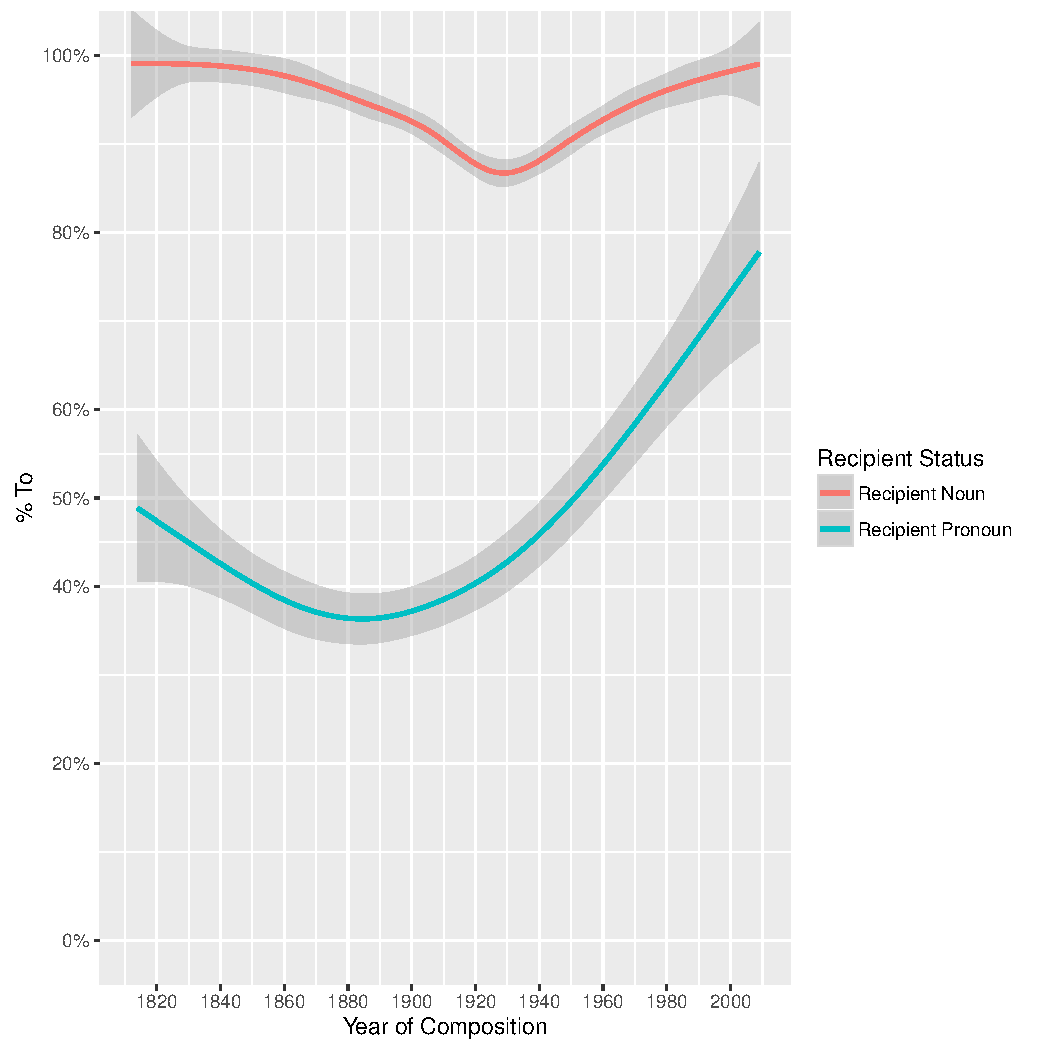
\includegraphics[width=\linewidth]{../images/directtheme-am}
		\caption{LOESS curves showing the loss of direct theme passivisation with GIVE and OFFER in American English}
		\label{fig:loss-of-dt-in-amen}
	\end{figure}

	The change in the locality properties of T and why that might occur is discussed further in the next subsection as part of a discussion of passivisation rates and the interplay between grammar learnability and language production. In particular, I discuss possible non-grammatical reasons for the rise in direct theme passivisation in the late 19th/early 20th century (especially seen with recipient nouns in Figure \ref{fig:loss-of-dt-in-amen}). Before turning to that, it is worthwhile to spend a brief moment on the loss of recipient pronoun cliticisation. As can be seen in Figure \ref{fig:loss-of-dt-in-amen}, direct theme passives are much more common with pronoun recipients than full noun phrase recipients, suggesting that pronoun cliticisation was a common operation that could independently derive direct theme passivisation. The higher rates of direct theme passivisation with recipient pronouns can be directly attributed in this case to the fact that there are two independent mechanisms for generating the same surface phenomenon. In the next subsection, the rate at which these mechanisms are used is discussed.
	
	In Chapter \ref{ch:passive}, I showed that direct theme passivisation survived in American English after the loss of theme cliticisation (i.e., after sentences like ``I gave it him'' became ungrammatical). While the loss of theme cliticisation and the loss of recipient cliticisation were shown to not be identical, there is a plausible connection between the two. It is plausible that language learners generalise evidence about one type of cliticisation, using the evidence of cliticisation with one type of pronoun as supporting evidence for cliticisation with other types of pronouns. Thus, the loss of theme cliticisation removed a potential source of evidence for the existence of cliticisation in the grammar. It is probably not coincidental that direct theme passivisation begins to decline around the same time that theme cliticisation is lost (i.e., 1940s).

	\subsection{Changes in Use of Grammar}

	This subsection discusses a change in American English with respect to the rate of passivisation of ditransitive sentences, especially considering the rates of passivisation of theme--recipient and recipient--theme clauses separately. By passivisation rate for theme--recipient and recipient--theme clauses, I refer to the number of passive sentences with a theme--recipient order (i.e., theme passivisation) out of all theme--recipient sentences (i.e., the number of theme passives divided by the number of theme passives plus the number of theme--recipient actives). For recipient--theme clauses, the same calculation was done, but with recipient passives and recipient--theme actives. In discussing these rates, I start with the end point of the change (i.e., Modern American English), which represents the expected relationship between grammar and use. I then show that this expected relationship is a recent development in the history of English. I then discuss the situation in prior stages of English and argue that is should be accounted for by an non-grammatical mechanism rather than trying to account for the change in patterns with a change in the grammar.

	Assuming that passivisation is pragmatically motivated (probably relating to demotion of agents), it should be expected that passivisation rates should be fairly stable across grammatical contexts. In particular, given that the difference between recipient and theme passivisation does not affect the pragmatic motivation for passivisation (i.e., does not impact the need to demote the subject) and given that both recipient and theme passivisation are grammatical, a naive prediction would be that passivisation rates among recipient--theme and theme--recipient clauses should be roughly equivalent (i.e., the rate of passivisation should be independent of the choice between recipient--theme and theme--recipient word order). Indeed, in late 20th and 21st century American English, this prediction holds; the rate of passivisation in recipient--theme and theme--recipient contexts are roughly equivalent. Collapsing GIVE and OFFER data after 1950, the passivisation rate in recipient--theme contexts is 5.9\%, while the passivisation rate in theme--recipient contest is 5.4\%.\footnote{This result was calculated from the hand-coded data discussed in Chapter \ref{ch:passive} from COHA. The hand coded data included only a sample of active and passive clauses. On the assumption that the sample was representative of the relative portion of recipient--theme and theme--recipient clauses (for both actives and passives), I automatically extracted the number of active and passives sentences with GIVE and OFFER. I then distributed the active and passive sentences into recipient--theme and theme--recipient groups based on the proportions from the hand coded samples. Then passivisation rates for each group was calculated. According to a chi-square test, the two conditions are independent (when looking at the data from 1950 onwards), but there is so much data that essentially any difference would be statistically significant.}
	
	This independence, however, is a new development in the history of English. Early American English and British English (up until the early 20th century) show a lack of independence between passivisation and word order. In particular, passivisation is much rarer in recipient--theme clauses than in theme--recipient clauses with the consequence that recipient passivisation is quite rare. That this property changed in American English can be seen in Figure \ref{fig:am-change-pass}.


	\begin{figure}[ht!]
		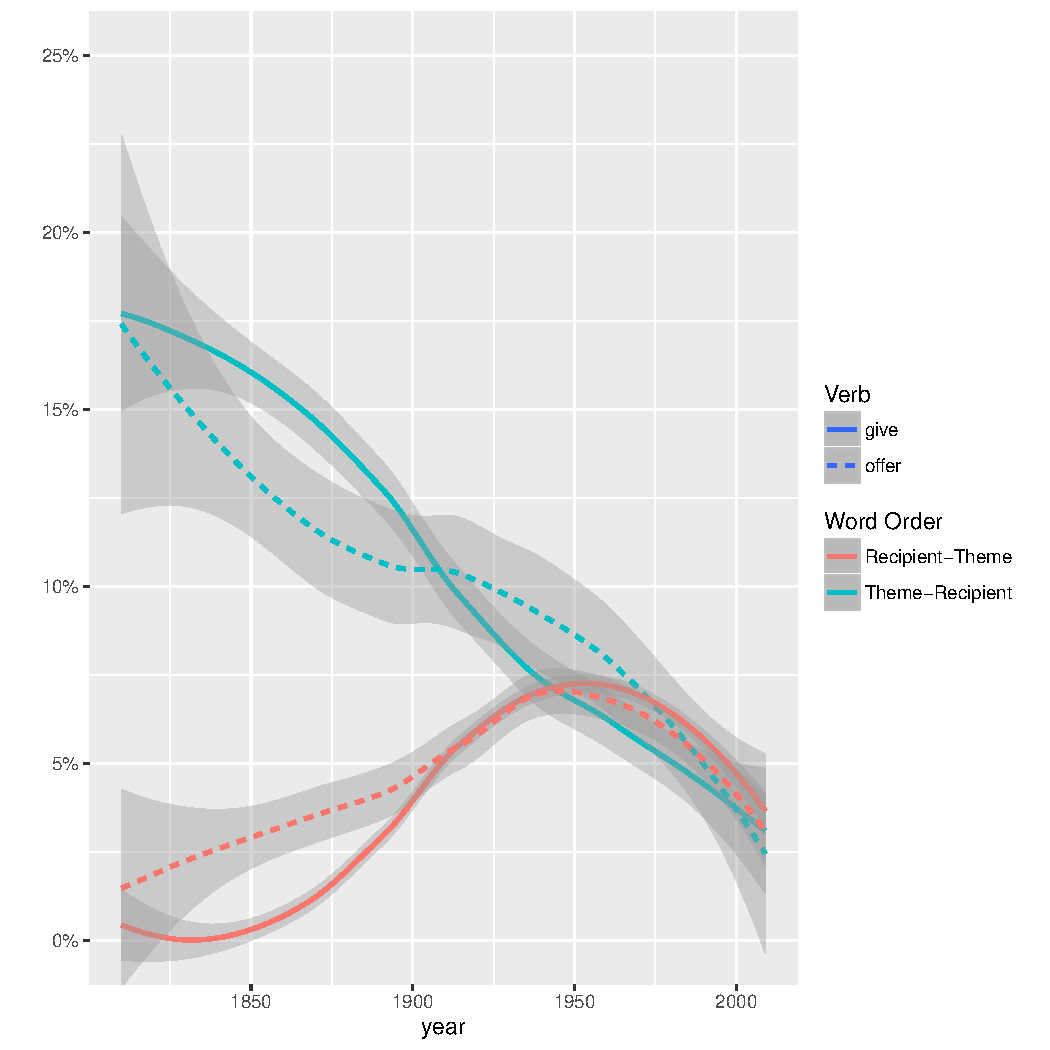
\includegraphics[width=\linewidth]{../images/am-change-pass}
		\caption{Rates of passivisation for GIVE and OFFER from COHA}
		\label{fig:am-change-pass}
	\end{figure}

	This depressed rate of passivisation in recipient--theme clauses has been a long time property of English. Using data from the Parsed Corpora of Historical English discussed in the previous section, the rate of passivisation in recipient--theme clauses was calculated for British English from 1200 (beginning of Middle English) until the 1910s (end of the corpora). The optimal logistic regression model (based on AIC) does not include an effect of year, indicating that the passivisation rate in recipient--theme clauses was stably low ($\sim$1\% of all recipient--theme clauses) for over 700 years. 

	At the same time, passivisation in theme--recipient clauses was consistently (and significantly) higher than in recipient--theme clauses ($\sim$15\% of all theme--recipient clauses). As can be seen in Figure \ref{fig:brit-pas}, the rate in theme--recipient clauses is similar to the general rate of passivisation in the language, which was calculated by dividing the number of passive clauses (excluding pseudopassives) by the number of passive clauses (excluding pseudopassives) plus the number of active clauses with at least one object (i.e., clauses which could have been passivised). Since the passivisation rate in theme--recipient clauses is similar to the general passivisation rate, it is the lower rate in recipient--theme clauses that needs to be explained.

	\begin{figure}[ht!]
		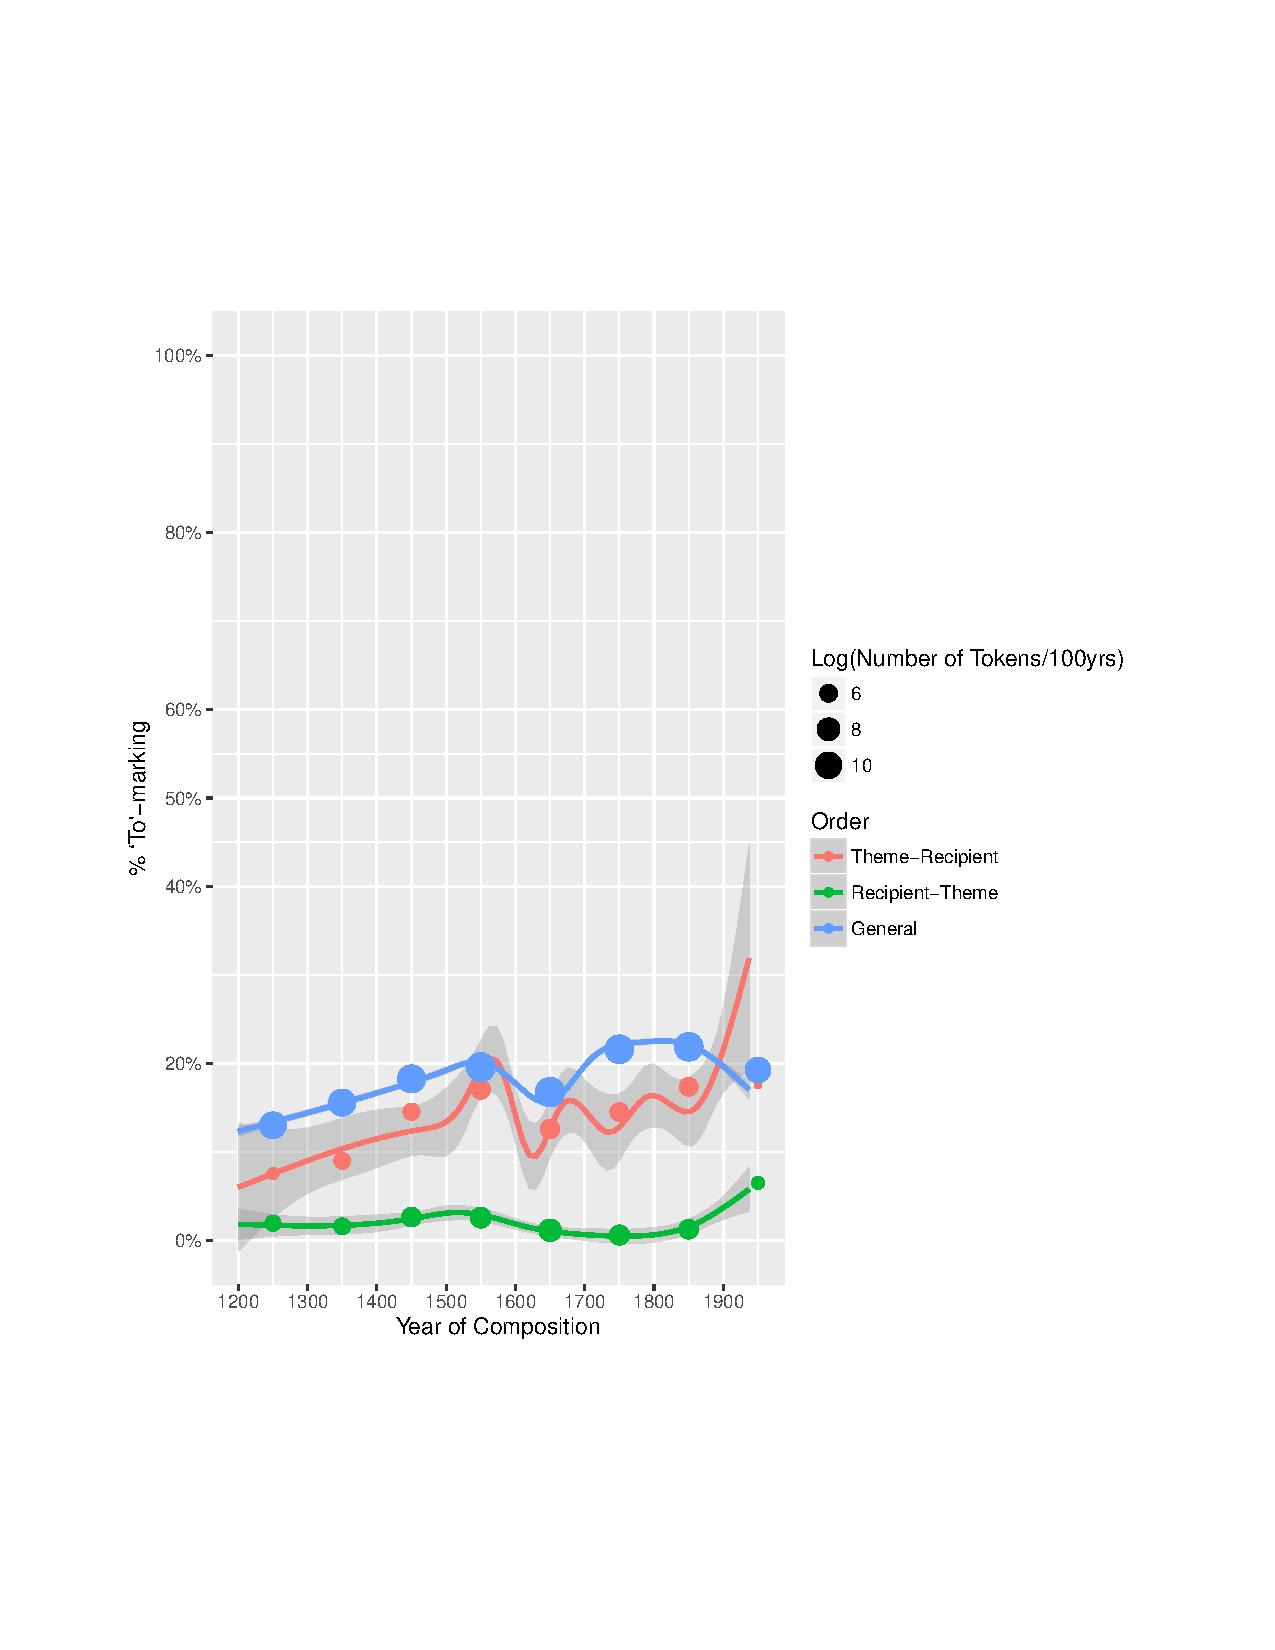
\includegraphics[width=\linewidth]{../images/brit-pas}
		\caption{LOESS fits for rates of passivisation in theme--recipient, recipient theme and general clauses}
		\label{fig:brit-pas}
	\end{figure}

	It would not be simple to provide a grammatical explanation for the phenomenon. In spite of being rarer, recipient passivisation appears to be grammatical (rather than being the artifact of production errors), since an occurrence rate of 1\% seems high for production errors (especially errors involving swapping the position of two arguments). A more complex story would need to claim (as I did in the previous subsection discussing direct theme passivisation) that a difference in rates reflects different derivations for the same string (in the direct passivisation case, the derivations were through relativised minimality and recipient pronoun cliticisation). 
	
	However, passivisation itself is not thought to arise from multiple sources (i.e., it is the effect of a single change in a Voice functional head). In order for different grammatical sources to derive this change, the logic would require that recipient--theme passivisation \textbf{lacks} some passivisation operation that all other clauses share. This is in parallel to the direct theme passive case; direct theme passivisation was higher with recipient pronouns, because there were two different ways of deriving the effect (relativised minimality and recipient pronoun cliticisation). A grammatical explanation of rate differences suggests that higher rates reflects more operations for deriving the relevant construction. Since I already showed that when the rates for recipient--theme passivisation increase in American English, it only increases to become identical to the rates in theme--recipient orders, this would mean that all other passive clauses have some mechanism for passivisation that the recipient--theme order lacks. I am unable to think what such a mechanism would be.

	In addition to not having a viable candidate for a grammatical operation, there is another reason to think that the depressed rate is not grammatical, namely, that the grammar of recipient passivisation changes during the relevant period without affecting the depressed rates. As discussed in the previous subsection, recipient passivisation changed from having oblique recipients to nominative recipients during the period from 1200 to about 1500. At this same time, the rate of recipient passivisation stayed the same. If the rate of recipient passivisation was being driven by grammatical factors, it seems implausible that a change in the relevant grammar would not influence the rate.

	This raises the obvious question: what would a non-grammatical explanation look like? Here is where it is important to separate linguistic competence into grammatical and non-grammatical components. As discussed in the introduction to this chapter, the grammar provides the possibilities to the speaker, but another linguistic component is responsible for determining the probability distribution over those possibilities. Under this conception, the formalisation of the depressed rate is simple: there is an interaction between passivisation and argument order in ditransitives (with passivisation less likely with recipient--theme orders). 

	While this provides a formal mechanism for capturing the phenomenon, it does not constitute an explanation. Why is there such an interaction? What constraints are there on interactions? Are interactions of this type common or rare? While a full discussion of the nature of the probability component would require another dissertation, I include here a brief discussion of possible answers to the first question (the reasons for the interaction). 

	It is worthwhile to note that the marked nature of recipient passives is found across Germanic languages. Icelandic allows theme passivisation even though theme--recipient word orders are ungrammatical in the active. Oblique subjects are extremely rare cross-linguistically, and P-incorporation also appears to be a marked operation (as seen by the rarity of pseudopassivisation). Language users seem to prefer to not manipulate PPs in order to have them become subjects. In cases where there is no other alternative (e.g., pseudopassives), speakers use P-incorporation to accomplish their goals. However, when there are other options available (e.g., theme passivisation for ditransitives), speakers avoid using a grammatical alternative involving manipulating a PP unless other factors (e.g., information structure) force them to use P-incorporation (or allow oblique subjects). 

	Returning to direct theme passivisation can give some further insight into the nature of the formal interaction. Since direct theme passivisation is (by definition) theme passivisation from the recipient--theme order, it should fall under the scope of the interaction (i.e., it should also show a decreased rate). Indeed, direct theme passivisation with full noun phrase recipients is quite rare ($\sim$2\% of all theme passives with full noun phrase recipients). However, direct theme passivisation is quite common with pronominal recipients (~50\% of all theme passives with pronominal recipients). This discrepancy in rates between full noun phrases and pronouns is informative about what triggers the interaction (i.e., non-cliticised recipients adjacent to the voice morpheme).

	In addition, the change in the non-grammatical system for determining passivisation rates for recipient--theme clauses explains the initial rise in direct theme passivisation in late 19th and early 20th century American English (shown in the previous subsection). Since direct theme passivisation (especially with full noun phrase recipients) derives from passivisation of recipient--theme clauses, increase in the rates of recipient--theme clause passivisation also increases the rate of direct theme passivisation. While this explains the initial rise in direct theme passivisation, it does not explain the subsequent decline.
	
	In the previous subsection, I attributed the decline to a grammatical change in the type of T heads available in the language (does T treat PPs as invisible for subjecthood or as defective interveners). Possibly, the subsequent decline of direct theme passivisation with full noun phrase recipients was initiated by the grammatically unrelated decline in direct theme passivisation with recipient pronouns. That decline is attributable to a loss of recipient cliticisation, but language learners may have overgeneralised the loss of direct theme passives in these cases to apply to all sources of direct theme passivisation, leading them to posit a grammar where direct theme passivisation was banned across the board (the grammar where PPs are defective interveners).

\section{Conclusions}
	In this chapter, I showed examples of using quantitative studies in syntactic change to inform linguistic research. This was embedded in a discussion of the nature of linguistic architecture and the relevance of different types of linguistic evidence. Examples were brought to show that quantitative use data can be informative about grammar, but is essential in studying systematic non-grammatical aspects of language.
	
	Looking at the development of recipient marking in English (i.e., the innovation of `to' as the marker of recipients) provided an example of how even complex changes involving the interaction of two distinct changes can be broken apart using relatively simple statistical processes. By breaking apart interacting changes, it is possible to use quantitative measures (such as the Constant Rate Effect) to study the grammatical architecture underlying each change. In this case, the initial rise of `to' as a marker of recipients showed a Constant Rate Effect implying that there was one underlying `to' grammar. On the other hand, the development of a null allomorph (used when the recipient is adjacent to the verb) showed a significant interaction between year and recipient status (pronoun vs. noun), indicating that the null allomorphy reflects different underlying grammars for nouns and pronouns. While this finding is not surprising, given the already known differences between nouns and pronouns in English morphology, it could not have been discovered without looking at quantitative data.
	
	Looking at passivisation, another case of a clear grammatical change was identified. In particular, both nominative recipient passivisation and pseudopassivasition increase in use during the same time period (Middle and Early Modern English). In this case, there was insufficient data to get quantitative results, but the qualitative overlap gives tentative support to the notion that both nominative recipient passivisation and pseudopassivisation are driven by the same mechanism (namely P-incorporation).

	Finally, the second case study also provided some insight into the underlying mechanism driving changes in use frequency of syntactic mechanisms. In at least some cases, it is the mechanism for determining probability distributions for production that is subject to change. In this case, passivisation was less likely in recipient--theme clauses (independently of whether the passivisation would produce an oblique recipient subject, a nominative recipient subject or direct theme passivisation). This restriction was stable for almost 700 years, but in American English was lost in favour of the simpler system with a uniform passivisation rate across environments. This provided evidence for a non-grammatical component to language competence (a system for determining probabilities for production), which can most profitably be studied using corpora of production.

%\bibliography{diss}
